\subsection{Definition}

Linear programming consist of a maximisation of a linear fonction subject to linear constraints.

\subsubsection{Example}

\begin{tabular}{m{8cm}m{5cm}}
    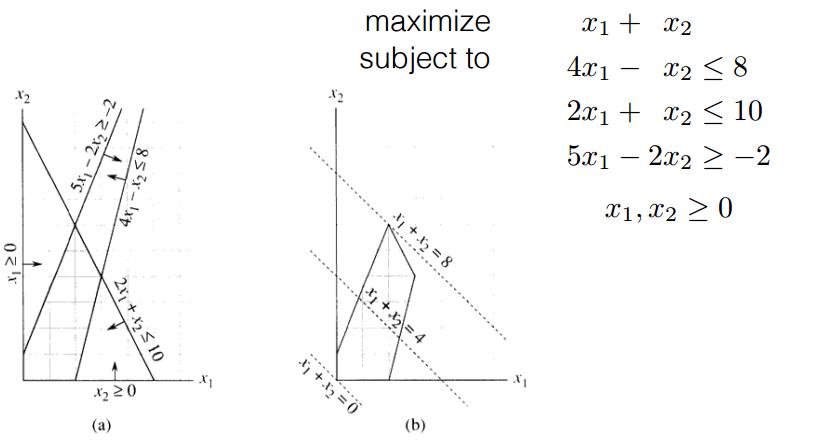
\includegraphics[width=7cm]{example1.png}
    &
    \begin{eqnarray*}
        \textrm{maximize } & x_1 + x_2 \\
        \textrm{subject to } & 4x_1 - x_2 \leq 8 \\
                           & 2x_1 + x_2 \leq 10 \\
                            & 5x_1 - 2x_2 \geq -2\\
                            & x_1, x_2 \geq 0
        \end{eqnarray*}
\end{tabular}

\subsection{Polytope}

The solution space is a \textbf{polytope}. In a polytope, every point is a convex
combination of its vertices:
$$(\alpha x + (1 - \alpha)y) \in S \, \quad  with \quad \, \alpha \in
[0,1]$$

\begin{tabular}{m{8cm}m{4cm}}
    \begin{eqnarray*}
        \textrm{maximize } & c_1x_1 + ... + c_nx_n \\
        \textrm{subject to } & a_{11}x_1 + ... + a_{1n}x_n \leq b_1 \\
                             & ... \\
                             & a_{m1}x_1 + ... + a_{mn}x_n \leq b_m \\
        \end{eqnarray*}
        &
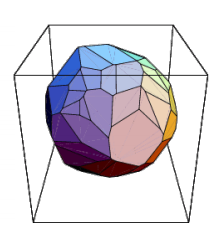
\includegraphics[width=3cm]{polytope.png}
\end{tabular}


\subsubsection{Theorem}
At least one of the points where the objective value is maximal is a vertex of the polytope.
\paragraph{Proof} : 
\begin{itemize}
    \item The maximum $x^{*}$ as a combination of the vertices of the
        polytope $v_{1},...,v_{t}$)
        $$x^{*} = \lambda_{1} v_{1} + ... + \lambda_{t} v_{t}$$

    \item Objective value at optimality can be expressed as a scalar
        product with $c$ a vector
        and the objective value at optimality can be expressed as a scalar product (c is a vector)
        $$c x^{*} = \lambda_{1} * (cv_{1}) + ... + \lambda_{t} * (cv_{t})$$
\end{itemize}

Let's assume that the maximum is not a vertex (each vertex is less good than $x^{*}$) \\
$$cx^{*} > cv_{i} \quad \forall i : 1 \leq i \leq t$$
Then we have 
\begin{align*}
cx^{*} =& \, \lambda_{1} * (cv_{1}) + ... + \lambda_{t} * (cv_{t}) \\
<& \, \lambda_{1} * (cx^{*}) + ... + \lambda_{t} * (cx^{*}) \\
<& \, (\lambda_{1} + ... + \lambda_{t}) (cx^{*}) \\
<& \, cx^{*}
\end{align*}

$\Rightarrow $ With this contradiction we can see that the maximal
$x^{*}$ must be a vertex.

\subsubsection{Algorithm}
We know that the best solution is located on a vertex of the
polytope:
\begin{enumerate}

    \item A naive approach would be to enumerate every vertices and take
        the one with the larget value. But, the problem is that the
        number of vertice grow exponentially with the number of
        inequality. 

    \item A better approach is the simplex algorithm. The idea is to
        move from one vertex to another with an improving objective
        function. We know this to be optimal thanks to the convexity of
        the polytope.
\end{enumerate}

\subsection{Simplex Algorithm}

\subsubsection{Standard and slack forms}
In order to use the simplex algorithm we need to transform our linear problem to a standard form (non negativity constraint on all the variable and replace equality to inequality) then to a slack form (introduction of basis variable in order to find a Basic Feasible Solution).

\centerline{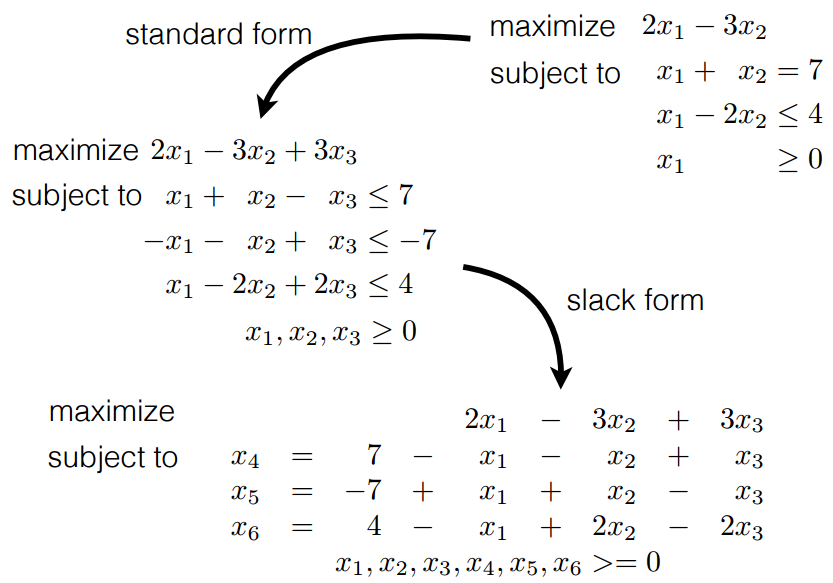
\includegraphics[scale=0.5]{staslack.png}}

\subsubsection{Basic Feasible Solution}
When our problem is represented as a slack we can find a BFS. We set every non basic variable to 0, we then get the value of our basis variable and an objective set to 0. Now the simplex algorithm will improve this solution with the pivot.

Sometimes the slack form won't return a BFS easily because some basics variables will be less than 0. In order to find a BFS with this kind of slack form, we need to put all the variables to the right such that you have $0 = constraints ...$ you then replace 0 in each constraint with a new variable and minimize their sum. With this new construction you have a BFS to this modified problem. If you arrive at z = 0 then you have a BFS to the initial problem, else the problem is not feasible.

\subsubsection{Pivot}
Now that we have our BFS, can we improve this. We will increase our non basics variables and decrease the basics one. But we can not decrease the basics ones less than 0. So for every non basics variables that we will increase, we must check at what value we must stop in order to have no basics variables under 0.

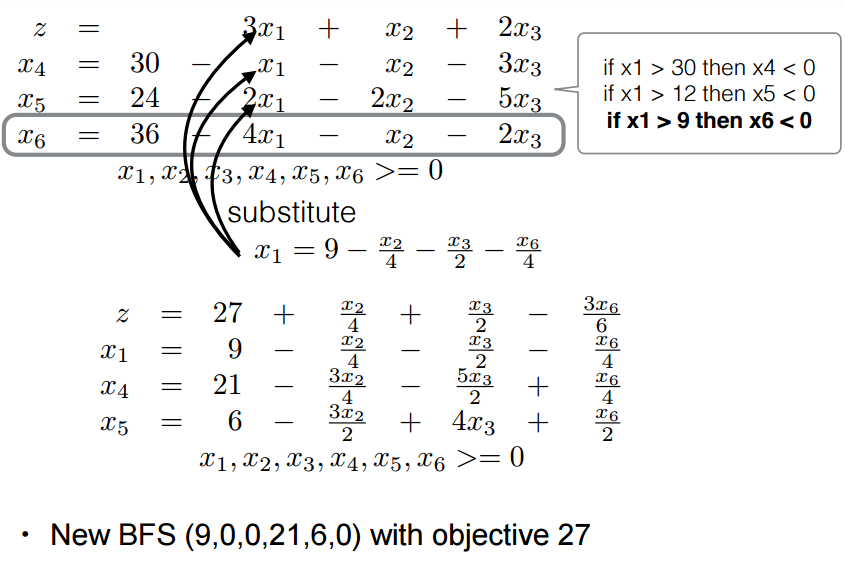
\includegraphics[scale=0.4]{pivot1.png}
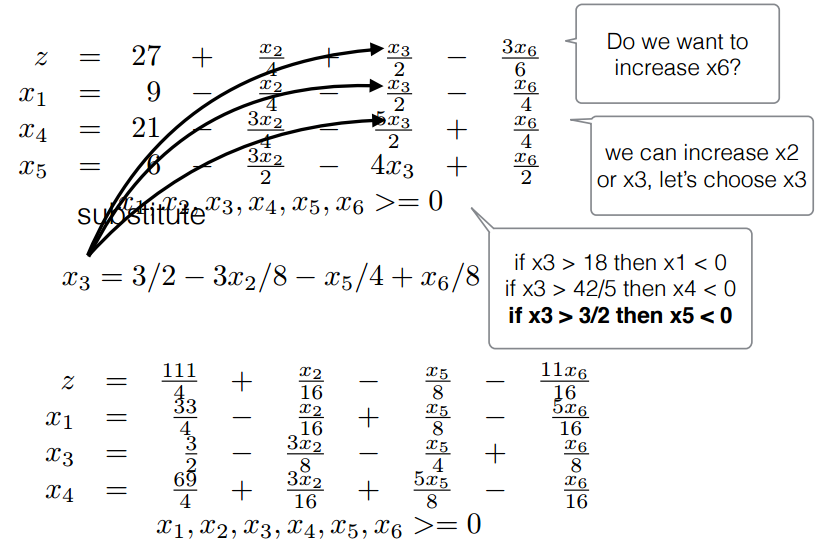
\includegraphics[scale=0.4]{pivot2.png}
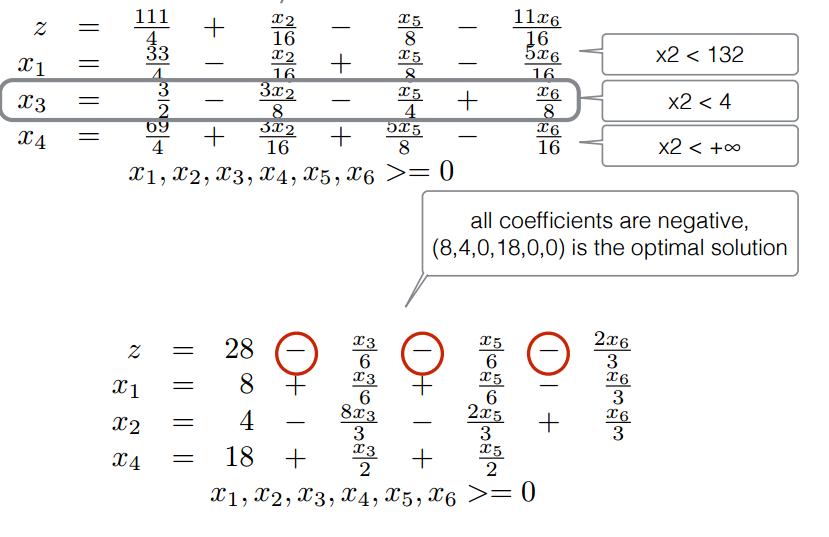
\includegraphics[scale=0.4]{pivot3.png}

\subsubsection{Cycling and degeneracy}
Sometimes an iteration will leaves the objective value unchanged (degeneracy). This can lead to cycling leaving us the same slack form at two different iterations. Those cycles can be avoided by breaking ties choosing the variables with the smallest index for example (Brand's rule). (Line 3 and 8 of the simplex algorithm).

\subsubsection{Limit of the simplex algorithm}
Most of the time the simplex algorithm performs very well. But it has been shown that on some particular problem we get a worst case scenario of exponential complexity. LP solving is not NP Hard, there exists other algorithm of polynomial complexity (Ellipsoid, Interior points). Those algorithms are not necessarily better than the simplex.

\subsection{Pseudo-code}

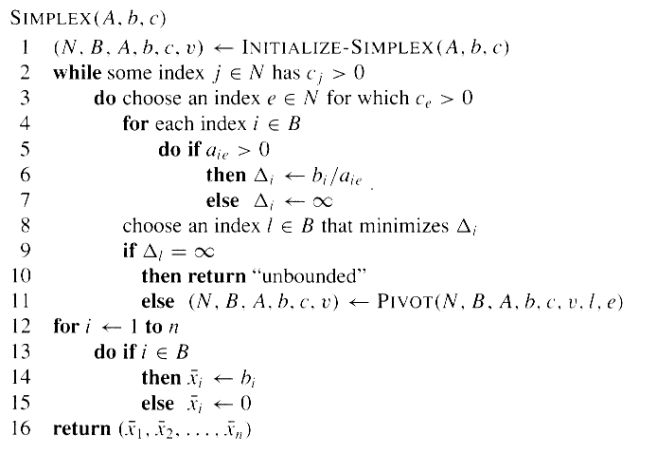
\includegraphics[scale=0.5]{simplex.png}
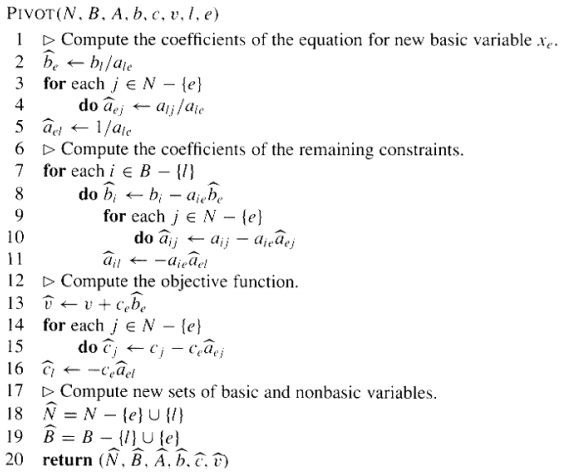
\includegraphics[scale=0.5]{pivot.png}

\subsection{Integer Linear Programming (NP-Hard)}

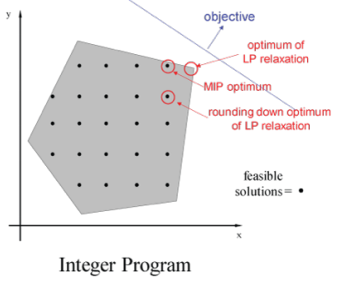
\includegraphics[scale=0.5]{integerlinearprogram.png}
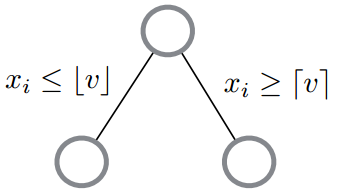
\includegraphics[scale=0.5]{branch.png}

We can solve this using branch and bounds. If at the optimal solution of the linear programming relaxation, one variable is not an integer xi = v, we create two branches and adding those constraints will only decrease the upper-bound.

\subsection{What is expected of you !}
Formulate a linear program. \\
Be able to transform a LP into standard and slack form. \\
Explain and be able to find a initial BFS. \\
Apply the simplex algorithm on a small example. (be familiar with the pivoting)\\
Explain how to detect an unbounded objective.
